\documentclass[11pt]{article}

% ----------------------------------------------------------------------
%  A-to-Z primer:
%  Uniform Spanning Trees, Loop-Erased Random Walks, Wilson's Algorithm,
%  Winding, and Random Environments (Extension 3)
% ----------------------------------------------------------------------

\usepackage[a4paper,margin=2.4cm]{geometry}
\usepackage{amsmath,amssymb,amsthm}
\usepackage{microtype}
\usepackage{booktabs}
\usepackage{enumitem}
\usepackage{tikz}
\usepackage{pgfplots}
\pgfplotsset{compat=1.18}
\usepgfplotslibrary{groupplots}
\usetikzlibrary{arrows.meta,positioning,calc,decorations.pathreplacing,backgrounds}
\usepackage[colorlinks=true,linkcolor=blue!55!black,citecolor=teal!55!black,
            urlcolor=blue!55!black]{hyperref}

% ---- colours -----------------------------------------------------------
\definecolor{walkcol}{RGB}{30,110,200}
\definecolor{lerwcol}{RGB}{200,60,40}
\definecolor{treecol}{RGB}{30,140,80}
\definecolor{gridcol}{RGB}{170,170,180}
\definecolor{accent}{RGB}{150,80,170}
\definecolor{boxbg}{RGB}{245,247,250}

% ---- theorem environments ---------------------------------------------
\theoremstyle{definition}
\newtheorem{definition}{Definition}[section]
\newtheorem{example}{Example}[section]
\newtheorem{remark}{Remark}[section]
\theoremstyle{plain}
\newtheorem{theorem}{Theorem}[section]
\newtheorem{proposition}{Proposition}[section]

% ---- handy macros ------------------------------------------------------
\newcommand{\Z}{\mathbb{Z}}
\newcommand{\E}{\mathbb{E}}
\newcommand{\Var}{\operatorname{Var}}
\newcommand{\LE}{\mathrm{LE}}
\newcommand{\BL}{B_{L}}
\newcommand{\Wind}{W_{L}}

\title{\bfseries Uniform Spanning Trees, Loop-Erased Random Walks,\\
and Random Environments\\[4pt]
\large A complete from-scratch primer for the Extension 3 project}
\author{Project primer prepared for Alberto Rescigno\\
\small Supervised project with Prof.\ Sunil Chhita, Durham University}
\date{\today}

\begin{document}
\maketitle

\begin{abstract}
\noindent
This document is a self-contained, A-to-Z introduction to everything you need
in order to understand and work on this project, starting from the bare basics
(what a graph and a random walk are) and building up to the precise research
experiment you will run: simulating loop-erased random walks in a fixed random
environment and measuring how the \emph{winding} of the path scales with the
size of the box. It is meant to be read linearly. Every new object is defined,
motivated, and illustrated with a figure before it is used. The final sections
state the precise experiment, the central question
($C\log L$ versus $C(\log L)^2$), and the pitfalls to watch for.
\end{abstract}

\tableofcontents
\bigskip

% ======================================================================
\section{The big picture: what this project is about}
% ======================================================================

Before any definitions, here is the whole project on one page.

\begin{itemize}[leftmargin=1.4em]
  \item We work on a \textbf{grid} of points (a finite chunk of the integer
        plane $\Z^2$).
  \item A \textbf{random walker} starts at the centre and hops between
        neighbouring points at random.
  \item If we delete the loops the walker makes, we get a clean
        self-avoiding path: a \textbf{loop-erased random walk} (LERW).
  \item Doing this repeatedly until every point is connected gives a
        \textbf{uniform spanning tree} (UST); the recipe is
        \textbf{Wilson's algorithm}.
  \item The path from the centre to the edge \emph{wraps around} the centre
        a certain amount. We call this its \textbf{winding}.
  \item In the usual symmetric case the winding fluctuates with variance
        $\Var(\Wind)\sim C\log L$. The new idea (\textbf{Extension 3}) is to
        make each point of the grid \emph{biased at random} --- a
        \textbf{random environment} --- and ask whether the winding now
        fluctuates more, perhaps like $C(\log L)^2$.
\end{itemize}

Figure~\ref{fig:roadmap} shows how the objects fit together. The arrows are
the operations; read it left to right.

\begin{figure}[h]
\centering
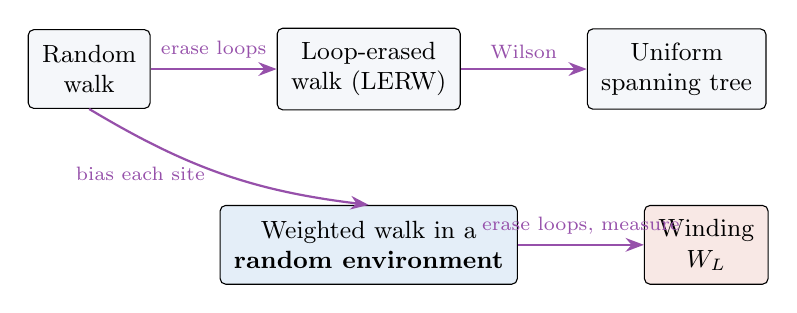
\begin{tikzpicture}[
   node distance=6mm and 16mm,
   box/.style={draw,rounded corners=2pt,fill=boxbg,inner sep=5pt,
               minimum height=10mm,align=center,font=\small},
   op/.style={->,>=Stealth,thick,accent}]
  \node[box] (rw)  {Random\\walk};
  \node[box,right=of rw] (lerw) {Loop-erased\\walk (LERW)};
  \node[box,right=of lerw] (ust) {Uniform\\spanning tree};
  \node[box,below=12mm of lerw,fill=walkcol!12] (env)
        {Weighted walk in a\\\textbf{random environment}};
  \node[box,right=of env,fill=lerwcol!12] (wind) {Winding\\$\Wind$};

  \draw[op] (rw) -- node[above,font=\scriptsize]{erase loops} (lerw);
  \draw[op] (lerw) -- node[above,font=\scriptsize]{Wilson} (ust);
  \draw[op] (rw.south) to[bend right=12]
        node[left,font=\scriptsize,xshift=-1mm]{bias each site} (env.north);
  \draw[op] (env) -- node[above,font=\scriptsize]{erase loops, measure} (wind);
\end{tikzpicture}
\caption{Map of the objects. The top row is the classical theory; the bottom
row is the Extension 3 experiment. The single new ingredient is replacing the
symmetric walk by a walk that is randomly biased at every site.}
\label{fig:roadmap}
\end{figure}

% ======================================================================
\section{Graphs and the square lattice}
% ======================================================================

\begin{definition}[Graph]
A \emph{graph} $G=(V,E)$ is a set of \emph{vertices} $V$ together with a set of
\emph{edges} $E$, where each edge joins two vertices. Two vertices are
\emph{neighbours} (or \emph{adjacent}) if an edge joins them.
\end{definition}

Our graph is a finite piece of the integer plane.

\begin{definition}[Square grid / lattice]
The \emph{integer lattice} is $\Z^2=\{(i,j): i,j\in\Z\}$. Two points are
neighbours when they differ by one in exactly one coordinate, i.e.
$(i,j)\sim(i',j')$ iff $|i-i'|+|j-j'|=1$. A finite \emph{grid graph} is the
induced subgraph on a finite box of such points.
\end{definition}

Each interior point has four neighbours, in the four compass directions
\textbf{N, E, S, W}. Figure~\ref{fig:grid} shows a $5\times5$ grid.

\begin{figure}[h]
\centering
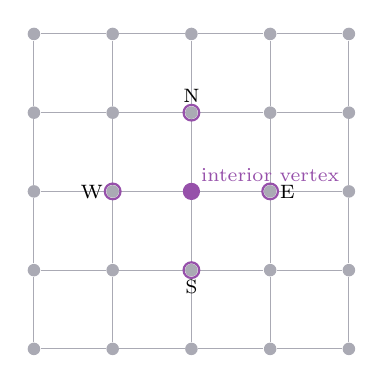
\begin{tikzpicture}[scale=1.0,
   v/.style={circle,fill=gridcol,inner sep=1.6pt}]
  \foreach \x in {0,...,4}{
    \foreach \y in {0,...,4}{
      \node[v] (n\x\y) at (\x,\y) {};
    }}
  \foreach \x in {0,...,4}{
    \foreach \y in {0,...,3}{
      \draw[gridcol] (n\x\y)--(n\x\the\numexpr\y+1\relax);
    }}
  \foreach \y in {0,...,4}{
    \foreach \x in {0,...,3}{
      \draw[gridcol] (n\x\y)--(n\the\numexpr\x+1\relax\y);
    }}
  % highlight an interior vertex and its four neighbours
  \node[circle,fill=accent,inner sep=2.2pt] (c) at (2,2) {};
  \foreach \nb in {(2,3),(3,2),(2,1),(1,2)}{
     \node[circle,draw=accent,thick,inner sep=2pt] at \nb {};}
  \node[font=\scriptsize,accent,above right] at (2,2) {interior vertex};
  \node[font=\scriptsize,above] at (2,3) {N};
  \node[font=\scriptsize,right] at (3,2) {E};
  \node[font=\scriptsize,below] at (2,1) {S};
  \node[font=\scriptsize,left]  at (1,2) {W};
\end{tikzpicture}
\caption{A $5\times5$ grid graph. The highlighted interior vertex has four
neighbours, labelled by compass direction.}
\label{fig:grid}
\end{figure}

\begin{definition}[Spanning tree]
A \emph{tree} is a connected graph with no cycles. A \emph{spanning tree} of a
connected graph $G$ is a subgraph that (i) includes \emph{every} vertex of $G$,
(ii) is connected, and (iii) has no cycles. A spanning tree on $|V|$ vertices
always has exactly $|V|-1$ edges.
\end{definition}

A finite connected graph generally has astronomically many spanning trees; the
exact number is given by Kirchhoff's \emph{Matrix-Tree theorem}. Choosing one
of them \emph{uniformly at random} is the central object of Section~5.

% ======================================================================
\section{Random walks}
% ======================================================================

\begin{definition}[Simple symmetric random walk]
A walker sits at a vertex. At each step it moves to one of the neighbouring
vertices chosen \emph{uniformly at random}. On the interior of the square grid
there are four neighbours, so
\[
   p_N=p_E=p_S=p_W=\tfrac14 .
\]
\end{definition}

\begin{figure}[h]
\centering
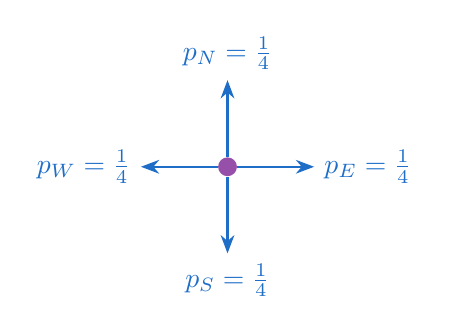
\begin{tikzpicture}[scale=1.1,>=Stealth]
  \node[circle,fill=accent,inner sep=2.4pt] (c) at (0,0) {};
  \node[font=\small] at (0,-0.05) {};
  \draw[->,walkcol,thick] (c)--(0,1)   node[above]{$p_N=\tfrac14$};
  \draw[->,walkcol,thick] (c)--(1,0)   node[right]{$p_E=\tfrac14$};
  \draw[->,walkcol,thick] (c)--(0,-1)  node[below]{$p_S=\tfrac14$};
  \draw[->,walkcol,thick] (c)--(-1,0)  node[left]{$p_W=\tfrac14$};
\end{tikzpicture}
\caption{The symmetric walk: from an interior site each of the four directions
is equally likely.}
\label{fig:srw}
\end{figure}

\begin{remark}[Recurrence]
A deep fact (Pólya's theorem) is that the simple random walk on $\Z^2$ is
\emph{recurrent}: it returns to its starting point infinitely often, and it
visits every site eventually. This is why the walk makes loops, and why loop
erasure (next section) is needed to extract a clean path.
\end{remark}

On a finite box we run the walk until it first reaches the boundary. Because
$\Z^2$ is recurrent, a typical walk visits many sites repeatedly, producing a
tangled trajectory like the blue path in Figure~\ref{fig:loop-erase}(left).

% ======================================================================
\section{Loop-erased random walk (LERW)}
% ======================================================================

The walk itself is full of loops. We turn it into a \emph{self-avoiding} path
by erasing loops as soon as they close, in chronological order.

\begin{definition}[Loop erasure]
Given a path $\gamma=(X_0,X_1,\dots,X_m)$, walk along it in time order. Whenever
you arrive at a vertex you have visited before, delete the entire loop between
the previous visit and now. The result $\LE(\gamma)$ visits no vertex twice ---
it is \emph{self-avoiding}.
\end{definition}

\begin{example}[Erasing one loop]
Suppose the walk visits
\[
   A \to B \to C \to D \to B \to E .
\]
When it returns to $B$, the loop $B\to C\to D\to B$ is erased, leaving
$A\to B\to E$. The order matters: we always keep the \emph{earliest} visit to a
vertex.
\end{example}

\begin{figure}[h]
\centering
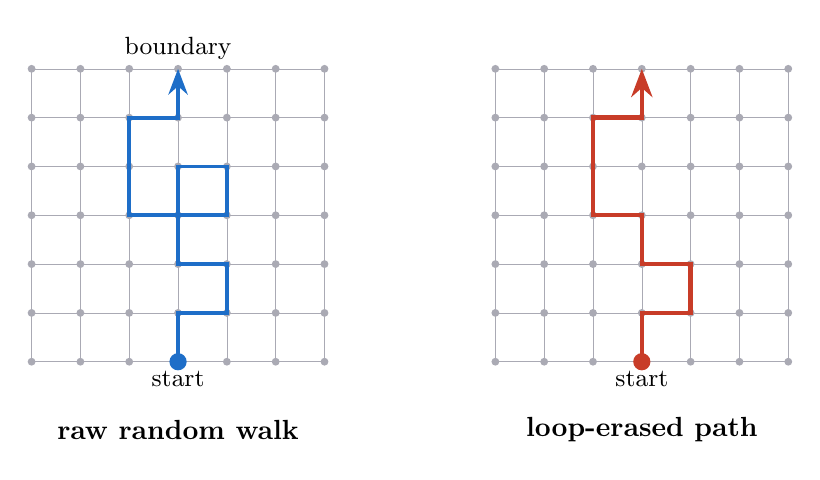
\begin{tikzpicture}[scale=0.62,
   v/.style={circle,fill=gridcol,inner sep=1.0pt}]
  % ---------- left panel: raw walk with a loop ----------
  \begin{scope}
    \foreach \x in {0,...,6}\foreach \y in {0,...,6}{\node[v] at (\x,\y){};}
    \foreach \x in {0,...,6}\foreach \y in {0,...,5}
        {\draw[gridcol,very thin](\x,\y)--(\x,\the\numexpr\y+1\relax);}
    \foreach \y in {0,...,6}\foreach \x in {0,...,5}
        {\draw[gridcol,very thin](\x,\y)--(\the\numexpr\x+1\relax,\y);}
    % raw walk (contains a loop around (3,3))
    \draw[walkcol,line width=1.4pt,->,>=Stealth]
      (3,0)--(3,1)--(4,1)--(4,2)--(3,2)--(3,3)--(4,3)--(4,4)--(3,4)--(3,3)
      --(2,3)--(2,4)--(2,5)--(3,5)--(3,6);
    \node[circle,fill=walkcol,inner sep=2.2pt] at (3,0){};
    \node[font=\small,below] at (3,0) {start};
    \node[font=\small,above] at (3,6) {boundary};
    \node[font=\bfseries] at (3,-1.4) {raw random walk};
  \end{scope}
  % ---------- right panel: loop-erased ----------
  \begin{scope}[xshift=9.5cm]
    \foreach \x in {0,...,6}\foreach \y in {0,...,6}{\node[v] at (\x,\y){};}
    \foreach \x in {0,...,6}\foreach \y in {0,...,5}
        {\draw[gridcol,very thin](\x,\y)--(\x,\the\numexpr\y+1\relax);}
    \foreach \y in {0,...,6}\foreach \x in {0,...,5}
        {\draw[gridcol,very thin](\x,\y)--(\the\numexpr\x+1\relax,\y);}
    \draw[lerwcol,line width=1.6pt,->,>=Stealth]
      (3,0)--(3,1)--(4,1)--(4,2)--(3,2)--(3,3)
      --(2,3)--(2,4)--(2,5)--(3,5)--(3,6);
    \node[circle,fill=lerwcol,inner sep=2.2pt] at (3,0){};
    \node[font=\small,below] at (3,0) {start};
    \node[font=\bfseries] at (3,-1.4) {loop-erased path};
  \end{scope}
\end{tikzpicture}
\caption{Left: a raw walk from the start to the boundary; it makes a loop near
the centre. Right: after chronological loop erasure the path is self-avoiding.}
\label{fig:loop-erase}
\end{figure}

\begin{remark}
In two dimensions the LERW has a beautiful scaling limit: rescaled, it converges
to a random fractal curve called $\mathrm{SLE}_2$ (Schramm--Loewner evolution
with parameter $\kappa=2$), and its paths have Hausdorff dimension $5/4$. You do
not need this to run the simulations, but it is the reason the winding has a
clean predicted scaling (Section~8).
\end{remark}

% ======================================================================
\section{Uniform spanning trees and Wilson's algorithm}
% ======================================================================

\begin{definition}[Uniform spanning tree (UST)]
The \emph{uniform spanning tree} of a finite connected graph is a spanning tree
chosen \emph{uniformly at random} among all spanning trees: every spanning tree
is equally likely.
\end{definition}

How do we sample one efficiently, without listing all (astronomically many)
spanning trees? Wilson's algorithm does exactly this using loop-erased walks.

\begin{figure}[h]
\centering
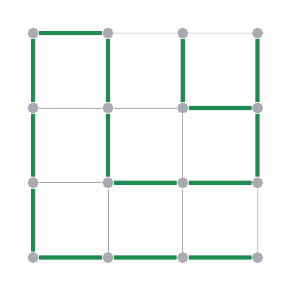
\begin{tikzpicture}[scale=0.95,v/.style={circle,fill=gridcol,inner sep=1.4pt}]
  \foreach \x in {0,...,3}\foreach \y in {0,...,3}{\node[v] (n\x\y) at (\x,\y){};}
  \foreach \x in {0,...,3}\foreach \y in {0,...,2}
     {\draw[gridcol,very thin](n\x\y)--(n\x\the\numexpr\y+1\relax);}
  \foreach \y in {0,...,3}\foreach \x in {0,...,2}
     {\draw[gridcol,very thin](n\x\y)--(n\the\numexpr\x+1\relax\y);}
  % a valid spanning tree: 16 vertices, exactly 15 edges, no cycle
  \draw[treecol,line width=1.5pt]
     (n00)--(n10)--(n20)--(n30)
     (n00)--(n01)--(n02)--(n03)--(n13)--(n12)--(n11)--(n21)--(n31)--(n32)--(n33)
     (n32)--(n22)--(n23);
\end{tikzpicture}
\caption{One spanning tree of a $4\times4$ grid: 16 vertices, 15 edges, no
cycles, every vertex connected. A UST is one such tree chosen uniformly.}
\label{fig:tree}
\end{figure}

\paragraph{Wilson's algorithm.}
\begin{enumerate}[leftmargin=2em,itemsep=2pt]
  \item Pick a \emph{root} vertex $r$ and start the tree as $T=\{r\}$.
  \item While some vertex is not yet in $T$:
    \begin{enumerate}[label=(\alph*)]
       \item pick any vertex $x$ not in $T$;
       \item run a random walk from $x$ until it first \emph{hits} $T$;
       \item loop-erase that walk;
       \item add the loop-erased path to $T$.
    \end{enumerate}
  \item Return $T$.
\end{enumerate}

\begin{theorem}[Wilson, 1996]
For the simple symmetric random walk, Wilson's algorithm returns a sample of the
\emph{uniform} spanning tree, regardless of the order in which vertices are
chosen.
\end{theorem}

\begin{figure}[h]
\centering
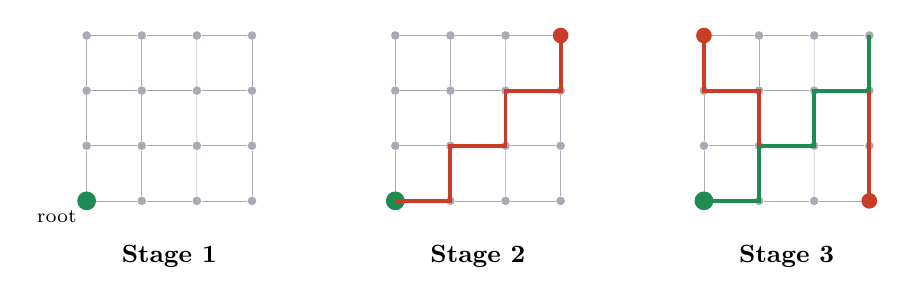
\begin{tikzpicture}[scale=0.7,v/.style={circle,fill=gridcol,inner sep=1.1pt}]
  \foreach \p/\lab in {0/Stage 1,5.6/Stage 2,11.2/Stage 3}{
   \begin{scope}[xshift=\p cm]
    \foreach \x in {0,...,3}\foreach \y in {0,...,3}
       {\node[v] (n\x\y) at (\x,\y){};}
    \foreach \x in {0,...,3}\foreach \y in {0,...,2}
       {\draw[gridcol,very thin](n\x\y)--(n\x\the\numexpr\y+1\relax);}
    \foreach \y in {0,...,3}\foreach \x in {0,...,2}
       {\draw[gridcol,very thin](n\x\y)--(n\the\numexpr\x+1\relax\y);}
    \node[font=\small\bfseries] at (1.5,-1) {\lab};
   \end{scope}}
  % stage 1: just the root
  \node[circle,fill=treecol,inner sep=2.4pt] at (0,0){};
  \node[font=\scriptsize,below left] at (0,0) {root};
  % stage 2: root + first LE branch
  \begin{scope}[xshift=5.6cm]
    \node[circle,fill=treecol,inner sep=2.4pt] at (0,0){};
    \draw[lerwcol,line width=1.4pt] (3,3)--(3,2)--(2,2)--(2,1)--(1,1)--(1,0)--(0,0);
    \node[circle,fill=lerwcol,inner sep=2pt] at (3,3){};
  \end{scope}
  % stage 3: more branches added
  \begin{scope}[xshift=11.2cm]
    \node[circle,fill=treecol,inner sep=2.4pt] at (0,0){};
    \draw[treecol,line width=1.4pt] (3,3)--(3,2)--(2,2)--(2,1)--(1,1)--(1,0)--(0,0);
    \draw[lerwcol,line width=1.4pt] (0,3)--(0,2)--(1,2)--(1,1);
    \draw[lerwcol,line width=1.4pt] (3,0)--(3,1)--(3,2);
    \node[circle,fill=lerwcol,inner sep=2pt] at (0,3){};
    \node[circle,fill=lerwcol,inner sep=2pt] at (3,0){};
  \end{scope}
\end{tikzpicture}
\caption{Wilson's algorithm building up. Stage 1: only the root (green). Stage
2: a loop-erased branch (red) is run from a new vertex until it hits the tree.
Stage 3: further branches are attached. Repeat until every vertex is included.}
\label{fig:wilson}
\end{figure}

\begin{proposition}[The single fact we exploit]
The unique path between two vertices in a UST has the same distribution as the
loop-erased random walk between them. Consequently, to study the branch from the
centre to the boundary, \textbf{we do not need the whole tree} --- it suffices
to run one walk from the centre to the boundary and loop-erase it. This is the
key efficiency of Extension 3.
\end{proposition}

\paragraph{Boundary conditions.}
Two conventions appear in the project. In the \emph{ordinary} finite grid the
boundary is just the outer ring of vertices. In the \emph{wired} version, all
boundary vertices are merged into a single root node (often called
\textsc{wire}); branches are then viewed as heading to one common absorbing
boundary (Figure~\ref{fig:wired}).

\begin{figure}[h]
\centering
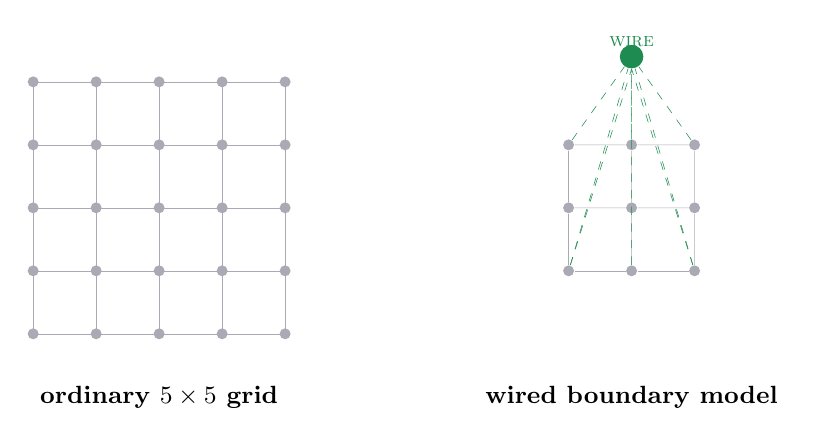
\begin{tikzpicture}[scale=0.8,v/.style={circle,fill=gridcol,inner sep=1.4pt}]
  \begin{scope}
    \foreach \x in {0,...,4}\foreach \y in {0,...,4}{\node[v] at (\x,\y){};}
    \foreach \x in {0,...,4}\foreach \y in {0,...,3}
       {\draw[gridcol,very thin](\x,\y)--(\x,\the\numexpr\y+1\relax);}
    \foreach \y in {0,...,4}\foreach \x in {0,...,3}
       {\draw[gridcol,very thin](\x,\y)--(\the\numexpr\x+1\relax,\y);}
    \node[font=\small\bfseries] at (2,-1) {ordinary $5\times5$ grid};
  \end{scope}
  \begin{scope}[xshift=7.5cm]
    % interior 3x3 only, boundary collapsed
    \foreach \x in {1,2,3}\foreach \y in {1,2,3}{\node[v] (m\x\y) at (\x,\y){};}
    \foreach \x in {1,2,3}\foreach \y in {1,2}
       {\draw[gridcol,very thin](m\x\y)--(m\x\the\numexpr\y+1\relax);}
    \foreach \y in {1,2,3}\foreach \x in {1,2}
       {\draw[gridcol,very thin](m\x\y)--(m\the\numexpr\x+1\relax\y);}
    \node[circle,fill=treecol,inner sep=3pt] (W) at (2,4.4) {};
    \node[font=\scriptsize,above,treecol] at (W) {\textsc{wire}};
    \foreach \x in {1,2,3}{
       \draw[treecol,very thin,dashed] (m\x3)--(W);
       \draw[treecol,very thin,dashed] (m\x1)--(W.south);}
    \draw[treecol,very thin,dashed] (m11)--(W);
    \draw[treecol,very thin,dashed] (m31)--(W);
    \node[font=\small\bfseries] at (2,-1) {wired boundary model};
  \end{scope}
\end{tikzpicture}
\caption{Ordinary vs.\ wired boundary. In the wired model the entire boundary is
a single absorbing root node \textsc{wire}.}
\label{fig:wired}
\end{figure}

% ======================================================================
\section{Winding: the observable we measure}
% ======================================================================

The quantity at the heart of the project is the \emph{winding} of the
loop-erased branch from the centre. Intuitively it measures how much the path
spirals (turns left versus right) on its way out.

\begin{definition}[Step directions and turns]
Write the loop-erased path as $\eta=(\eta_0,\eta_1,\dots,\eta_m)$ with
$\eta_0=(0,0)$. Each step has a direction $d_i=\eta_{i+1}-\eta_i\in\{N,E,S,W\}$.
For each consecutive pair of steps $(d_i,d_{i+1})$:
\[
  \text{left turn} \mapsto +1,\qquad
  \text{right turn}\mapsto -1,\qquad
  \text{straight}  \mapsto 0 .
\]
A $U$-turn cannot occur in a self-avoiding path. The \textbf{winding} is
\[
   \Wind \;=\; \#\{\text{left turns}\}-\#\{\text{right turns}\}.
\]
\end{definition}

\begin{figure}[h]
\centering
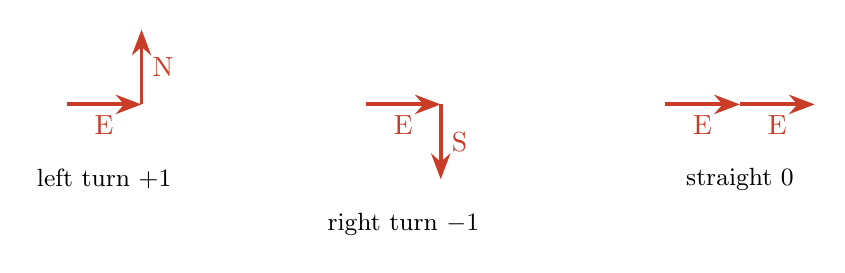
\begin{tikzpicture}[scale=0.95,>=Stealth]
  % left turn
  \begin{scope}
     \draw[lerwcol,line width=1.4pt,->] (0,0)--(1,0) node[midway,below]{E};
     \draw[lerwcol,line width=1.4pt,->] (1,0)--(1,1) node[midway,right]{N};
     \node[font=\small] at (0.5,-1) {left turn $+1$};
  \end{scope}
  % right turn
  \begin{scope}[xshift=4cm]
     \draw[lerwcol,line width=1.4pt,->] (0,0)--(1,0) node[midway,below]{E};
     \draw[lerwcol,line width=1.4pt,->] (1,0)--(1,-1) node[midway,right]{S};
     \node[font=\small] at (0.5,-1.6) {right turn $-1$};
  \end{scope}
  % straight
  \begin{scope}[xshift=8cm]
     \draw[lerwcol,line width=1.4pt,->] (0,0)--(1,0) node[midway,below]{E};
     \draw[lerwcol,line width=1.4pt,->] (1,0)--(2,0) node[midway,below]{E};
     \node[font=\small] at (1,-1) {straight $0$};
  \end{scope}
\end{tikzpicture}
\caption{The three turn types. Winding is the running total of $+1$ for left
turns and $-1$ for right turns.}
\label{fig:turns}
\end{figure}

\begin{example}[Winding of a small path]
Figure~\ref{fig:wind-path} shows a path that turns left three times and right
once, giving $\Wind=3-1=+2$. Equivalently, encode directions as
$E=0,N=1,W=2,S=3$ (counterclockwise). Then for consecutive codes,
$(d_{i+1}-d_i)\bmod 4 = 1$ is a left turn and $=3$ is a right turn --- this is
exactly how the code computes it.
\end{example}

\begin{figure}[h]
\centering
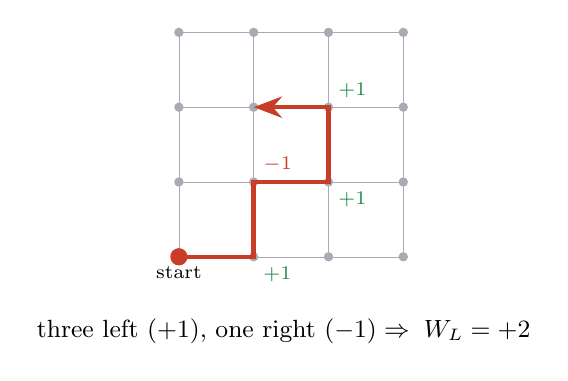
\begin{tikzpicture}[scale=0.95,>=Stealth,v/.style={circle,fill=gridcol,inner sep=1.2pt}]
  \foreach \x in {0,...,3}\foreach \y in {0,...,3}{\node[v] at (\x,\y){};}
  \foreach \x in {0,...,3}\foreach \y in {0,...,2}
     {\draw[gridcol,very thin](\x,\y)--(\x,\the\numexpr\y+1\relax);}
  \foreach \y in {0,...,3}\foreach \x in {0,...,2}
     {\draw[gridcol,very thin](\x,\y)--(\the\numexpr\x+1\relax,\y);}
  % path: E, N, E, N, W  ->  turns: +1, -1, +1, +1  (net +2)
  \draw[lerwcol,line width=1.6pt,->]
     (0,0)--(1,0)--(1,1)--(2,1)--(2,2)--(1,2);
  \node[circle,fill=lerwcol,inner sep=2.2pt] at (0,0){};
  \node[font=\scriptsize,below] at (0,0) {start};
  \node[font=\scriptsize,treecol,below right] at (1,0) {$+1$};
  \node[font=\scriptsize,lerwcol,above right] at (1,1) {$-1$};
  \node[font=\scriptsize,treecol,below right] at (2,1) {$+1$};
  \node[font=\scriptsize,treecol,above right] at (2,2) {$+1$};
  \node[font=\small] at (1.4,-1)
     {three left ($+1$), one right ($-1$)$\;\Rightarrow\;\Wind=+2$};
\end{tikzpicture}
\caption{A path making three left turns and one right turn:
$\Wind=3-1=+2$. The winding counts net turning in units of right angles.}
\label{fig:wind-path}
\end{figure}

\begin{remark}[Why winding, and why $\log L$?]
Up to the constant $\pi/2$, $\Wind$ is the cumulative turning \emph{angle} of
the path. For conformally invariant curves like the LERW, the winding angle of
the tip at distance $L$ from the start behaves like a Gaussian whose variance
grows logarithmically in $L$. This is the source of the
$\Var(\Wind)\sim C\log L$ prediction, made precise by Schramm's analysis of
$\mathrm{SLE}_2$ and predicted earlier by Coulomb-gas arguments
(Section~8).
\end{remark}

% ======================================================================
\section{The central question: how does the winding variance scale?}
% ======================================================================

We run many independent trials, record the winding $\Wind$ each time, and
estimate its \emph{variance} as a function of the box size $L$. The whole
project hinges on distinguishing two candidate laws:
\[
  \boxed{\ \Var(\Wind)\;\approx\; a\,\log L + b\ }
  \qquad\text{versus}\qquad
  \boxed{\ \Var(\Wind)\;\approx\; a\,(\log L)^2 + b\ }.
\]

The trick to telling them apart: plot the measured variance against $\log L$ on
one axis and against $(\log L)^2$ on the other. The \emph{correct} law is the
one that comes out as a straight line (Figure~\ref{fig:scaling}).

\begin{figure}[h]
\centering
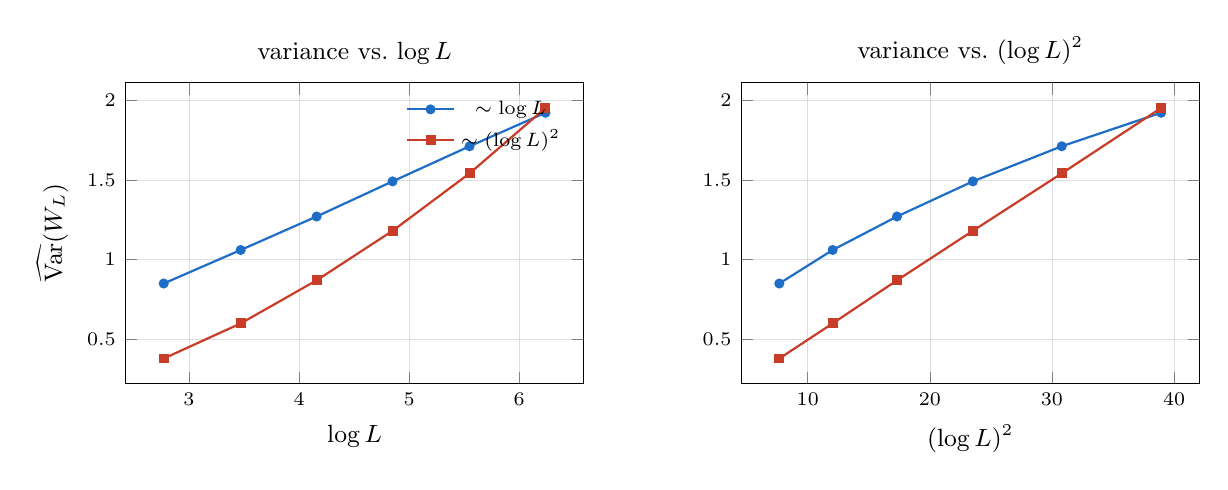
\begin{tikzpicture}
\begin{groupplot}[
   group style={group size=2 by 1, horizontal sep=2.0cm},
   width=7.4cm, height=5.4cm,
   tick label style={font=\scriptsize},
   label style={font=\small},
   legend style={font=\scriptsize,draw=none,fill=none},
   grid=both, grid style={gridcol!40,very thin},
]
% --- left: variance vs log L ---
\nextgroupplot[xlabel={$\log L$},ylabel={$\widehat{\Var}(\Wind)$},
   title={\small variance vs.\ $\log L$},title style={yshift=-1mm}]
  % linear-in-logL model: appears straight here
  \addplot[walkcol,thick,mark=*,mark size=1.4pt] coordinates
    {(2.77,0.85)(3.47,1.06)(4.16,1.27)(4.85,1.49)(5.55,1.71)(6.24,1.92)};
  \addlegendentry{$\sim\log L$}
  % quadratic-in-logL model: appears curved (convex) here
  \addplot[lerwcol,thick,mark=square*,mark size=1.4pt] coordinates
    {(2.77,0.38)(3.47,0.60)(4.16,0.87)(4.85,1.18)(5.55,1.54)(6.24,1.95)};
  \addlegendentry{$\sim(\log L)^2$}
% --- right: variance vs (log L)^2 ---
\nextgroupplot[xlabel={$(\log L)^2$},
   title={\small variance vs.\ $(\log L)^2$},title style={yshift=-1mm}]
  \addplot[walkcol,thick,mark=*,mark size=1.4pt] coordinates
    {(7.67,0.85)(12.04,1.06)(17.31,1.27)(23.52,1.49)(30.80,1.71)(38.94,1.92)};
  \addplot[lerwcol,thick,mark=square*,mark size=1.4pt] coordinates
    {(7.67,0.38)(12.04,0.60)(17.31,0.87)(23.52,1.18)(30.80,1.54)(38.94,1.95)};
\end{groupplot}
\end{tikzpicture}
\caption{Schematic of the discriminating plot (illustrative numbers, not real
data). A $\log L$ law is a straight line on the \emph{left} axis but curved on
the right; a $(\log L)^2$ law is straight on the \emph{right} axis but curved on
the left. Whichever panel linearises the data identifies the scaling.}
\label{fig:scaling}
\end{figure}

\begin{remark}[Three regimes to keep in mind]
\begin{enumerate}[leftmargin=1.6em,itemsep=2pt]
  \item \textbf{Symmetric} ($u=v=1$): the classical case, expected
        $\Var(\Wind)\sim C\log L$.
  \item \textbf{Mean-one random environment}: each site is biased at random but
        unbiased \emph{on average}. This is the open case --- it might stay
        $\log L$, or grow like $(\log L)^2$.
  \item \textbf{Genuine drift}: if the bias does not average out, the walk has a
        net direction and the winding variance can be \emph{finite} (it stops
        growing). Prof.\ Chhita noted this case explicitly.
\end{enumerate}
\end{remark}

% ======================================================================
\section{Random environments: the Extension 3 model}
% ======================================================================

The new ingredient is to make the walk biased differently at every site, with
the bias itself drawn at random and then \emph{frozen} for the whole walk.

\begin{definition}[Quenched vs.\ annealed]
A \emph{quenched} (fixed-in-time) environment is sampled \emph{once} and then
held fixed while the walk moves; the local probabilities at a site are the same
every time the walk visits it. An \emph{annealed} environment is resampled at
each step. \textbf{We use the quenched case} --- it is the more interesting one
and the one Prof.\ Chhita asked for.
\end{definition}

\paragraph{The edge-weight model.}
At each site $x$ sample two positive numbers $u_x,v_x>0$ and assign outgoing
\emph{edge weights}
\[
   w_N(x)=1,\quad w_E(x)=1,\quad w_S(x)=u_x,\quad w_W(x)=v_x .
\]
Then \emph{normalise} the weights into probabilities by dividing by their sum
$Z_x=2+u_x+v_x$:
\[
   p_N=\frac{1}{2+u_x+v_x},\quad
   p_E=\frac{1}{2+u_x+v_x},\quad
   p_S=\frac{u_x}{2+u_x+v_x},\quad
   p_W=\frac{v_x}{2+u_x+v_x}.
\]

\begin{figure}[h]
\centering
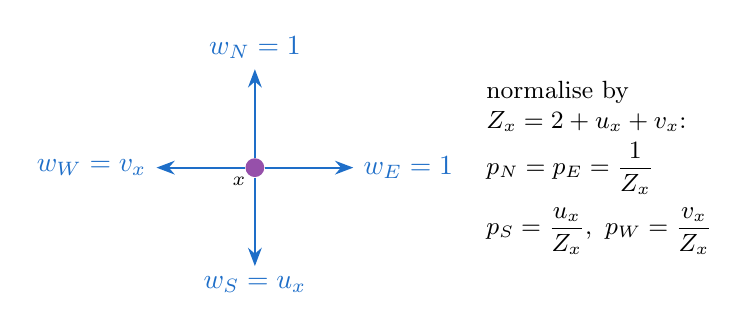
\begin{tikzpicture}[scale=1.25,>=Stealth]
  \node[circle,fill=accent,inner sep=2.4pt] (c) at (0,0) {};
  \node[font=\scriptsize,below left] at (c) {$x$};
  \draw[->,walkcol,thick] (c)--(0,1)   node[above]{$w_N=1$};
  \draw[->,walkcol,thick] (c)--(1,0)   node[right]{$w_E=1$};
  \draw[->,walkcol,thick] (c)--(0,-1)  node[below]{$w_S=u_x$};
  \draw[->,walkcol,thick] (c)--(-1,0)  node[left]{$w_W=v_x$};
  \node[font=\small,align=left] at (3.5,0)
     {normalise by\\$Z_x=2+u_x+v_x$:\\[3pt]
      $p_N=p_E=\dfrac{1}{Z_x}$\\[4pt]
      $p_S=\dfrac{u_x}{Z_x},\ p_W=\dfrac{v_x}{Z_x}$};
\end{tikzpicture}
\caption{A single site in the random environment. Two of the four directions
carry random weight; dividing by the total turns weights into probabilities.}
\label{fig:weighted-site}
\end{figure}

\begin{remark}[Why this is unbiased on average but biased per sample]
If $u_x,v_x$ have mean $1$, then $\E[w_N]=\E[w_E]=\E[w_S]=\E[w_W]=1$: the model
is symmetric \emph{on average}. But in any single frozen environment, some sites
push south or west more than others, creating a fixed pattern of local bias. It
is this frozen, spatially-correlated bias --- not a global drift --- that could
change the winding scaling.
\end{remark}

\paragraph{Choosing the disorder distribution.}
We need positive random variables with mean $1$. The cleanest choice is the
Gamma distribution with shape $k$ and scale $1/k$, written
$\mathrm{Gamma}(k,1/k)$, for which
\[
   \E[u_x]=1,\qquad \Var(u_x)=\frac1k .
\]
A large shape $k$ means weak disorder (close to the symmetric case); a small $k$
means strong disorder. The special value $k=1$ is the exponential distribution.
Figure~\ref{fig:gamma} shows several densities, all with mean $1$.

\begin{figure}[h]
\centering
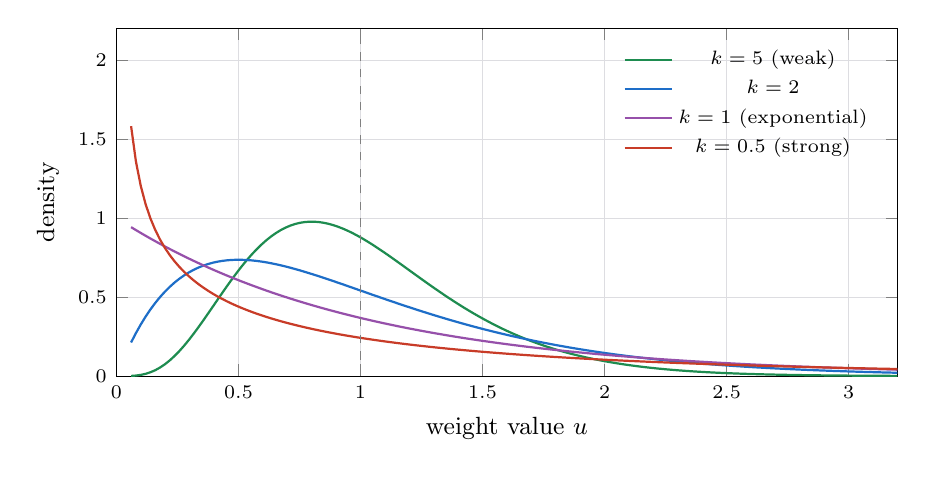
\begin{tikzpicture}
\begin{axis}[
   width=11.5cm, height=6.0cm,
   xlabel={weight value $u$}, ylabel={density},
   domain=0.06:3.2, samples=160,
   xmin=0,xmax=3.2, ymin=0, ymax=2.2,
   tick label style={font=\scriptsize}, label style={font=\small},
   legend style={font=\scriptsize,draw=none,fill=none,at={(0.98,0.97)},anchor=north east},
   grid=both, grid style={gridcol!40,very thin},
   restrict y to domain=0:5,
]
  % all densities are Gamma(shape=k, scale=1/k); mean 1, var 1/k
  % k=5:  x^4 e^{-5x} / (Gamma(5) * (1/5)^5),  Gamma(5)=24
  \addplot[treecol,thick] {x^4*exp(-5*x)/(24*(0.2)^5)};
  \addlegendentry{$k=5$ (weak)}
  % k=2:  x e^{-2x} / (Gamma(2)*(1/2)^2) = x e^{-2x}/0.25, Gamma(2)=1
  \addplot[walkcol,thick] {x*exp(-2*x)/(0.25)};
  \addlegendentry{$k=2$}
  % k=1:  exponential, e^{-x}
  \addplot[accent,thick] {exp(-x)};
  \addlegendentry{$k=1$ (exponential)}
  % k=0.5: x^{-0.5} e^{-0.5 x} / (Gamma(0.5)*2^{0.5}), Gamma(0.5)=1.7724539
  \addplot[lerwcol,thick] {x^(-0.5)*exp(-0.5*x)/(1.7724539*1.4142136)};
  \addlegendentry{$k=0.5$ (strong)}
  \draw[gray,dashed] (axis cs:1,0)--(axis cs:1,2.2);
  \node[gray,font=\scriptsize,anchor=south] at (axis cs:1,2.2) {mean $=1$};
\end{axis}
\end{tikzpicture}
\caption{Mean-one Gamma densities for several shape parameters $k$. Large $k$
concentrates near $1$ (weak disorder, nearly symmetric); small $k$ spreads out
and becomes heavy near $0$ (strong disorder).}
\label{fig:gamma}
\end{figure}

% ======================================================================
\section{Splitting the variance: where would anomalous scaling live?}
% ======================================================================

There is one mathematical identity that makes the whole experiment sharper. By
the \emph{law of total variance}, conditioning on the (frozen) environment
$\mathcal{E}$,
\[
   \Var(\Wind)
   \;=\;
   \underbrace{\E\!\big[\Var(\Wind\mid\mathcal{E})\big]}_{\text{within-environment (thermal)}}
   \;+\;
   \underbrace{\Var\!\big(\E[\Wind\mid\mathcal{E}]\big)}_{\text{between-environment (quenched)}} .
\]

The first term is the usual fluctuation of the walk inside a fixed landscape;
it should carry the classical $\log L$ behaviour. The second term measures how
much the \emph{typical} winding changes when you swap one frozen environment for
another. Any anomalous $(\log L)^2$ growth is most likely to appear in this
\emph{between-environment} term.

\begin{remark}[Practical pay-off]
You can estimate both terms directly: run $K>1$ independent walks inside
\emph{each} of $M$ frozen environments. The spread \emph{within} an environment
estimates the first term; the spread of the per-environment averages estimates
the second. With $K=1$ you only get the total. Designing the simulation with
$K>1$ costs almost nothing and tells you not just \emph{whether} the scaling
changes but \emph{why}. Figure~\ref{fig:decomp} sketches the expected picture.
\end{remark}

\begin{figure}[h]
\centering
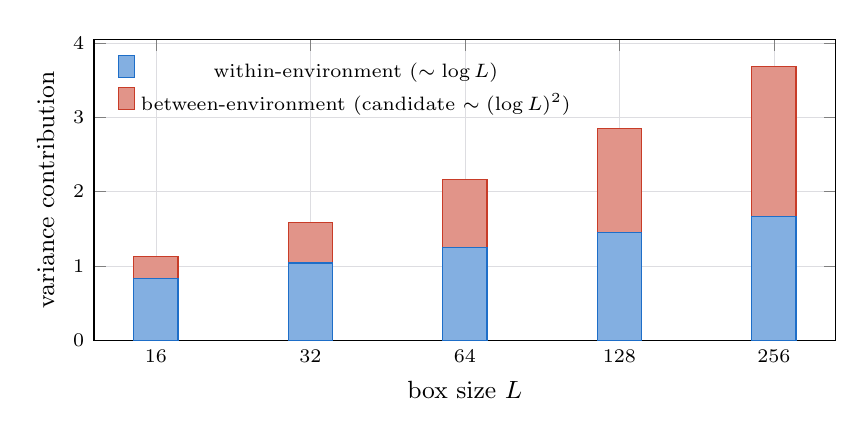
\begin{tikzpicture}
\begin{axis}[
   width=11cm, height=5.4cm,
   ybar stacked, bar width=16pt,
   xlabel={box size $L$}, ylabel={variance contribution},
   symbolic x coords={16,32,64,128,256},
   xtick=data, tick label style={font=\scriptsize}, label style={font=\small},
   legend style={font=\scriptsize,draw=none,fill=none,at={(0.02,0.97)},anchor=north west},
   ymin=0, grid=both, grid style={gridcol!40,very thin},
]
  % illustrative: within grows ~ log L, between grows faster
  \addplot[fill=walkcol!55,draw=walkcol] coordinates
    {(16,0.83)(32,1.04)(64,1.25)(128,1.45)(256,1.66)};
  \addlegendentry{within-environment ($\sim\log L$)}
  \addplot[fill=lerwcol!55,draw=lerwcol] coordinates
    {(16,0.30)(32,0.55)(64,0.92)(128,1.40)(256,2.02)};
  \addlegendentry{between-environment (candidate $\sim(\log L)^2$)}
\end{axis}
\end{tikzpicture}
\caption{Illustrative variance decomposition (not real data). If the
between-environment term grows faster than the within term, the total variance
bends upward from $\log L$ toward $(\log L)^2$ --- and you can see exactly which
piece is responsible.}
\label{fig:decomp}
\end{figure}

% ======================================================================
\section{The experiment, step by step}
% ======================================================================

Putting it together, one trial is:

\begin{enumerate}[leftmargin=2em,itemsep=2pt]
  \item Fix a box $\BL=[-L,L]^2\cap\Z^2$ with the origin at the centre.
  \item Sample a fresh quenched environment: draw $u_x,v_x$ for every interior
        site.
  \item Run the weighted walk from $(0,0)$ until it first hits the boundary
        $\partial\BL$.
  \item Loop-erase the path.
  \item Compute its winding $\Wind$.
  \item Record the trial (seed, $L$, distribution, parameter, walk length,
        LERW length, winding, hit location).
\end{enumerate}

Repeat over a grid of box sizes and disorder levels, then estimate, for each
pair $(L,k)$,
\[
   \overline{\Wind}=\frac1N\sum_{i=1}^N \Wind^{(i)},\qquad
   \widehat{\Var}(\Wind)=\frac{1}{N-1}\sum_{i=1}^N\big(\Wind^{(i)}-\overline{\Wind}\big)^2,
\]
and finally compare $\widehat{\Var}(\Wind)$ against $\log L$ and $(\log L)^2$.

\paragraph{Suggested ranges (start small, scale up).}
\begin{center}
\begin{tabular}{@{}lll@{}}
\toprule
Quantity & Debug & Serious run \\
\midrule
Box sizes $L$        & $16,32,64$            & $16,32,64,128,256\,(512)$ \\
Disorder $k$ (Gamma) & $1$                   & $20,10,5,2,1,0.5$ \\
Samples $N$ per $(L,k)$ & $50$--$100$        & $5000+$ if feasible \\
Walks per environment $K$ & $1$              & $1$, or $>1$ for the decomposition \\
\bottomrule
\end{tabular}
\end{center}

\paragraph{Pseudocode (for understanding, not to run yet).}
\begin{verbatim}
for each L:
  for each disorder level k:
    repeat N times:
      env  = sample_environment(L, k)        # quenched: fixed for this trial
      path = walk_from_origin_to_boundary(L, env)
      lerw = loop_erase(path)
      w    = winding(lerw)                    # left turns - right turns
      record(L, k, seed, len(path), len(lerw), w, hit)
\end{verbatim}

% ======================================================================
\section{Pitfalls to watch for}
% ======================================================================

\begin{itemize}[leftmargin=1.5em,itemsep=3pt]
  \item \textbf{Terminology.} Only the \emph{symmetric} case samples the
        \emph{uniform} spanning tree. Once the walk is weighted or
        site-dependent, say ``loop-erased random walk in a random environment''
        or ``random-walk-weighted spanning tree'' --- not ``UST''.
  \item \textbf{Mean-one is not the same as no drift.} Mean-one weights remove
        drift only \emph{on average}. Each frozen environment can still have
        local directional bias. Keep the quenched/annealed distinction crisp in
        write-ups (Section~10).
  \item \textbf{Boundary convention.} State the stopping rule explicitly (stop
        on first hitting $\partial\BL$) and never mix it silently with another
        convention; the winding depends on it.
  \item \textbf{Finite-size effects.} For small $L$ it is genuinely hard to tell
        $\log L$ from $(\log L)^2$. Use cautious wording: ``preliminary
        evidence,'' ``consistent with,'' ``not yet conclusive.''
  \item \textbf{Gamma parametrisation.} Use shape $k$ with scale $1/k$ so the
        mean is exactly $1$ and the variance is $1/k$. Getting the
        shape/scale convention wrong silently changes the disorder.
  \item \textbf{Reproducibility.} Seed every environment and every walk
        deterministically, so any run can be reproduced and any anomaly can be
        re-examined.
  \item \textbf{Cost.} The expected number of raw steps to exit a box of
        half-size $L$ grows like $L^2$, so large $L$ with many samples is
        expensive; budget accordingly and keep a defensive cap on walk length.
\end{itemize}

% ======================================================================
\section{Glossary}
% ======================================================================

\begin{description}[leftmargin=0pt,style=nextline,itemsep=2pt]
  \item[Random walk] A path that moves to a random neighbour at each step.
  \item[Loop erasure] Removing loops from a path in chronological order to make
        it self-avoiding.
  \item[LERW] Loop-erased random walk; the self-avoiding path obtained above.
  \item[Spanning tree] A cycle-free connected subgraph touching every vertex.
  \item[Uniform spanning tree (UST)] A spanning tree chosen uniformly at random.
  \item[Wilson's algorithm] Builds a UST by repeatedly adding loop-erased walks.
  \item[Wired boundary] All boundary vertices merged into one root node.
  \item[Winding $\Wind$] Number of left turns minus right turns along the path.
  \item[Random environment] Site-dependent transition bias, sampled once and
        frozen (quenched).
  \item[Quenched / annealed] Environment fixed for the walk / resampled each
        step.
  \item[Disorder parameter $k$] Controls the spread of the environment; here the
        Gamma shape, with variance $1/k$.
  \item[$C\log L$ scaling] Expected winding-variance growth in the symmetric
        case.
  \item[$C(\log L)^2$ scaling] Candidate growth to test in the random
        environment.
\end{description}

% ======================================================================
\section*{Further reading}
\addcontentsline{toc}{section}{Further reading}
% ======================================================================
\small
\begin{thebibliography}{9}
\bibitem{wilson} D.~B.~Wilson, \emph{Generating random spanning trees more
quickly than the cover time}, STOC 1996.
\bibitem{schramm} O.~Schramm, \emph{Scaling limits of loop-erased random walks
and uniform spanning trees}, Israel J.\ Math.\ \textbf{118} (2000), 221--288.
\bibitem{lsw} G.~F.~Lawler, O.~Schramm, W.~Werner, \emph{Conformal invariance of
planar loop-erased random walks and uniform spanning trees}, Ann.\ Probab.\
\textbf{32} (2004), 939--995.
\bibitem{ww} B.~Wieland, D.~B.~Wilson, \emph{Winding angle variance of
Fortuin--Kasteleyn contours}, Phys.\ Rev.\ E (2003) --- numerical study of
winding for SAW, LERW, FK contours and SLE.
\bibitem{lyonsperes} R.~Lyons, Y.~Peres, \emph{Probability on Trees and
Networks}, Cambridge University Press, 2016 --- standard reference for UST,
LERW, Wilson's algorithm.
\bibitem{lawler} G.~F.~Lawler, \emph{Intersections of Random Walks},
Birkh\"auser --- background on LERW.
\bibitem{kumagai} T.~Kumagai, \emph{Random Walks on Disordered Media and their
Scaling Limits}, Saint-Flour Lecture Notes in Mathematics \textbf{2101},
Springer, 2014 --- random walks in random environments.
\bibitem{rstre} Recent work on \emph{random spanning trees in random
environment} (e.g.\ Makowiec, Salvi and collaborators, 2024--2025), which
studies observables of spanning trees that interpolate between the UST and the
minimum spanning tree.
\end{thebibliography}

\end{document}